\documentclass[a4paper]{article}
\usepackage[utf8]{inputenc}
\usepackage[final]{graphicx}
\usepackage{amsmath} 
\usepackage{geometry}
\usepackage{appendix}
\usepackage{listings}
\usepackage{titling}
\usepackage{listings}
\usepackage{xcolor}

\definecolor{codegreen}{rgb}{0,0.6,0}
\definecolor{codegray}{rgb}{0.5,0.5,0.5}
\definecolor{codepurple}{rgb}{0.58,0,0.82}
\definecolor{codeblue}{rgb}{0,0,0.7}
\definecolor{backcolour}{rgb}{0.95,0.95,0.92}

\lstdefinestyle{mystyle}{
    backgroundcolor=\color{backcolour},   
    commentstyle=\color{codegreen},
    keywordstyle=\color{codeblue},
    numberstyle=\tiny\color{codegray},
    stringstyle=\color{codepurple},
    basicstyle=\ttfamily,
    breakatwhitespace=false,         
    breaklines=true,                 
    captionpos=b,                    
    keepspaces=true,                 
    numbers=left,                    
    numbersep=5pt,                  
    showspaces=false,                
    showstringspaces=false,
    showtabs=false,                  
    tabsize=2
}

\lstset{style=mystyle}

\newcommand{\subtitle}[1]{%
	\posttitle{%
		\par\end{center}
	\begin{center}\large#1\end{center}
	\vskip0.1em}}%
\graphicspath{{images/}}
\geometry{
 a4paper,
 margin=1in
}

\title{Project 1 Report}
\subtitle{CSS322 Scientific Computing\\Sirindhorn International Institute of Technology, Thammasat University\\Semester 1 Academic Year 2021}
\author{Paphana Yiwsiw 6222780379 (Section 3)}
\begin{document}
\maketitle
\tableofcontents
 
\section*{Answers for Part II}
\addcontentsline{toc}{section}{Answers for Part II}
\begin{figure}[h]
    \centering
    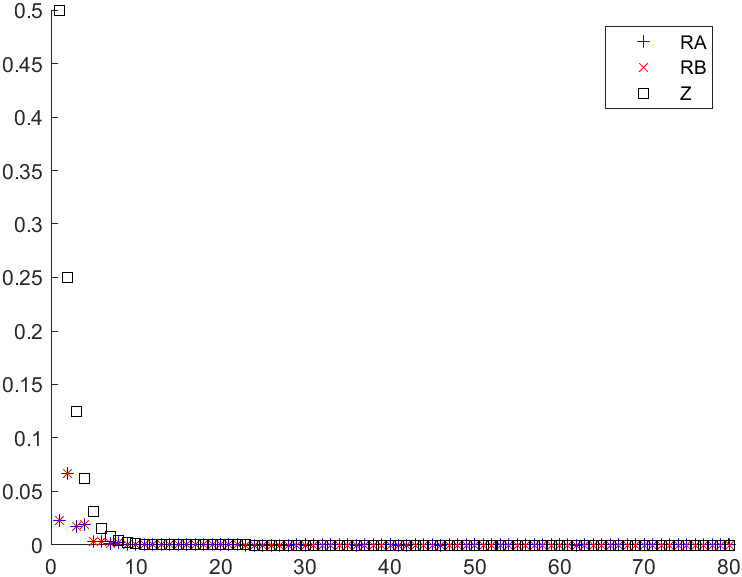
\includegraphics[width=10cm]{Part2_ScatterPlot.png}
    \caption{Scatter plots of diagonal elements of RA,RB,Z}
\end{figure}
After implementing QR factorization by Gram-Schmidt algorithm using both approaches given in part I of the project to the matrix A by given MATLAB commands, the approximation results of Gram-Schmidt-A and Gram-Schmidt-B is quite similar but it has a very small difference. But according to the observation, the approximation results from Gram-Schmidt-B version is more accurate than Gram-Schmidt-A by a small margin, possibly due to runoff.
\paragraph{}
The reason that caused difference in the result from implementations of part I is possibly due to how the value is updated in each loop. The main difference is at how it calculate the $r_{ij}$. In version A, it calculated by $r_{ji} = q_j^Ta_i$. But in version B, it was calculated by $r_{ij} = q_i^Tv_j$ in which making the accuracy to improve. Also, the order of accessing each entry is different. In the inner loop $j$, version A accessed from $1$ to $i-1$ but version B from $j+1$ to $n$. After all, it was calculated differently, thus making it has different result and some different may occurs due to runoff or even cancellation. 
 
\section*{Answers for Part III}
\addcontentsline{toc}{section}{Answers for Part III}
\paragraph{}
The matrix A that part III given is the special version of Toeplitz matrix, the upper triangular Toeplitz matrix where the main diagonal entry has the value of 1, the first upper superdiagonal has the value of 3, and the rest of the matrix has the value of 0. Hence, the matrix A of size nxn has the following form.

\begin{equation*}
A=
\begin{bmatrix}
   1 & 3 & 0 & \cdots & 0 \\
   0 & 1 & 3 & \cdots & 0 \\ 
   \vdots & \ddots & \ddots & \ddots & \vdots\\
   0 & \ddots &\ddots & 1 & 3 \\
   0 & \cdots &\cdots & 0 & 1\\
\end{bmatrix}
\end{equation*}


\subsection*{Rank of $A$}
\addcontentsline{toc}{subsection}{Rank of $A$}
\paragraph{}
Rank of matrix A is the number of linearly independent column of matrix A. From the given matrix, every column is unique and the determinant of matrix A is nonzero which will be discussed later. Thus, making it all linearly independent. Therefore, $rank(A) = n$, the number of column in the matrix A.

\subsection*{Determinant of $A$}
\addcontentsline{toc}{subsection}{Determinant of $A$}
\paragraph{}
Since the given matrix A is a upper triangular matrix. Hence, The determinant is the product of the main diagonal entry. Therefore, $det(A) = 1$

\subsection*{Eigenvalues of $A$}
\addcontentsline{toc}{subsection}{Eigenvalues of $A$}
\paragraph{}
To find the eigenvalues of the given matrix A, I used the characteristic polynomial equation, $det(A-\lambda I)=0$.
\begin{equation*}
A-\lambda I =
\begin{bmatrix}
   1-\lambda & 3 & 0 & \cdots & 0 \\
   0 & 1-\lambda & 3 & \cdots & 0 \\ 
   \vdots & \ddots & \ddots & \ddots & \vdots\\
   0 & \ddots &\ddots & 1-\lambda & 3 \\
   0 & \cdots &\cdots & 0 & 1-\lambda\\
\end{bmatrix}
\end{equation*}
\paragraph{}
As you can see, the matrix $A-\lambda I$ is still the upper triangular matrix. Thus, the $det(A-\lambda I)$ is also the product of main diagonal entry.
\begin{equation*}
\begin{split}
det(A-\lambda I) = (1-\lambda)^n &=0\\
1 - \lambda & = 0\\
\lambda &= 1    
\end{split}
\end{equation*}
\paragraph{}
Therefore, the eigenvalue of matrix A is 1.

\subsection*{Inverse of $A$}
\addcontentsline{toc}{subsection}{Inverse of $A$}
\paragraph{}
To find the inverse of the given matrix A, I used $A = P^{T}LU$ factorization. Then, reuse the factorization to solve for each column in the $A^{-1}$. Since, the given matrix A is already a upper triangular matrix and the product from two upper triangular matrices multiplication is also an upper triangular matrix. Thus, making $U = A$ and $P = L = I$ because $A=P^TLU=P^TL(A)=(I)(I)A=A$. Next, let $x_i$ denote the i-th column of $A^{-1}$ and $e_i$ denote the i-th column of $I_n$.
First, find $x_1$ by solving $Ax_1 = e_1$\\
Set,
\begin{equation*}
\begin{split}
\hat{e}_1 = Pe_1 &= Ie_1 = e_1 \\
\end{split}
\end{equation*}
Solve for $w_1$,
\begin{equation*}
\begin{split}
Lw_1 &= \hat{e}_1 \\
Iw_1 &= \hat{e}_1 \\
w_1 &= \hat{e_1} = e_1
\end{split}
\end{equation*}
Solve for $x_1$,
\begin{equation*}
\begin{split}
Ux_1 &= w_1 \\
Ax_1 &= e_1 \\
\begin{bmatrix}
   1 & 3 & 0 & \cdots & 0 \\
   0 & 1 & 3 & \cdots & 0 \\ 
   \vdots & \ddots & \ddots & \ddots & \vdots\\
   0 & \ddots &\ddots & 1 & 3 \\
   0 & \cdots &\cdots & 0 & 1\\
\end{bmatrix}
\begin{bmatrix}
   x_{1,1} \\ x_{1,2} \\ \vdots\\ \vdots\\ x_{1,n}
\end{bmatrix}
&= \begin{bmatrix}
   1 \\ 0 \\ \vdots\\ \vdots\\ 0
\end{bmatrix}\\
x_{1,n}, x_{1,n-1}, ... ,x_{1,2}&=0\\
x_{1,1} + 3x_{1,2} &=0\\
x_{1,1} &= 1\\
\end{split}
\end{equation*}
Thus, 
\begin{equation*}
\begin{split}
    x_1 &= \begin{bmatrix}
   1 \\ 0 \\ \vdots\\ \vdots\\ 0
        \end{bmatrix}\\
\end{split}
\end{equation*}
\paragraph{}
Next, solve for $x_2$.
\begin{equation*}
\begin{split}
\hat{e}_2 = Pe_2 = Ie_2 &= e_2 \\
Lw_2 = Iw_2 = w_2 = \hat{e}_2 &= e_2 \\
Ux_2 &= \hat{e}_2\\
Ax_2 &= e_2 \\
\begin{bmatrix}
   1 & 3 & 0 & \cdots & 0 \\
   0 & 1 & 3 & \cdots & 0 \\ 
   \vdots & \ddots & \ddots & \ddots & \vdots\\
   0 & \ddots &\ddots & 1 & 3 \\
   0 & \cdots &\cdots & 0 & 1\\
\end{bmatrix}
\begin{bmatrix}
   x_{2,1} \\ x_{2,2} \\ \vdots\\ \vdots\\ x_{2,n}
\end{bmatrix}
&= \begin{bmatrix}
   0 \\ 1 \\ 0\\ \vdots\\ 0
\end{bmatrix}\\
\end{split}
\end{equation*}
\paragraph{}
\begin{equation*}
\begin{split}
x_{2,n}, x_{2,n-1}, ... ,x_{2,3}&=0\\
x_{2,2} + 3x_{2,3} &=1\\
x_{2,2} &= 1\\
x_{2,1} + 3x_{2,2} &=0\\
x_{2,1} + 3(1) &=0 \\
x_{2,1} &= -3\\
    x_2 &= \begin{bmatrix}
   -3 \\ 1 \\ 0 \\ \vdots\\ 0
        \end{bmatrix}\\
\end{split}
\end{equation*}
\paragraph{}
Next, solve for $x_3$. Omitted the $\hat{e}_3$ and $Lw_3$ step since it has the same outcome of $\hat{e}_3 = w_3 = e_3$
\begin{equation*}
\begin{split}
Ux_3 &= \hat{e}_3\\
Ax_3 &= e_3 \\
\begin{bmatrix}
   1 & 3 & 0 & \cdots & 0 \\
   0 & 1 & 3 & \cdots & 0 \\ 
   \vdots & \ddots & \ddots & \ddots & \vdots\\
   0 & \ddots &\ddots & 1 & 3 \\
   0 & \cdots &\cdots & 0 & 1\\
\end{bmatrix}
\begin{bmatrix}
   x_{3,1} \\ x_{3,2} \\ \vdots\\ \vdots\\ x_{3,n}
\end{bmatrix}
&= \begin{bmatrix}
   0 \\ 0 \\ 1\\ \vdots\\ 0
\end{bmatrix}\\
x_{3,n}, x_{3,n-1}, ... ,x_{3,4}&=0\\
x_{3,3} + 3x_{3,4} &=1\\
x_{3,3} &= 1\\
x_{3,2} + 3x_{3,3} &=0\\
x_{3,2} + 3(1) &=0 \\
x_{3,2} &= -3\\
x_{3,1} + 3x_{3,2} &=0\\
x_{3,1} + 3(-3) &=0 \\
x_{3,1} &= 9\\
    x_3 &= \begin{bmatrix}
   9 \\ -3 \\ 1 \\ \vdots\\ 0
        \end{bmatrix}\\
\end{split}
\end{equation*}
\paragraph{}
To establish the pattern of $A^{-1}$ more clearly, the solved $x_4$ and $x_5$ is
\begin{equation*}
x_4 = \begin{bmatrix} -27 \\ 9 \\ -3 \\ 1 \\ 0 \\ \vdots\\ 0  \end{bmatrix},
x_5 = \begin{bmatrix} 81 \\ -27 \\ 9 \\ -3 \\ 1 \\ \vdots\\ 0  \end{bmatrix}
\end{equation*}
\paragraph{}
As you can see that the inverse of matrix A is also an upper triangular matrix. In the main diagonal entry has a value of 1. Then, in each i-th of upper superdiagonal entry has the value of $(-3)^i ,i = 1,2,..,n-1$. Thus, the inverse of given matrix A of size $nxn$ has this following form.
\begin{equation*}
A^{-1}=
\begin{bmatrix}
   1      & (-3)^1 & (-3)^2 & \cdots & \cdots & (-3)^{n-1}  \\
   0      & 1      & \ddots & \ddots &        & \vdots      \\
   \vdots & \ddots & \ddots & \ddots & \ddots & \vdots      \\
   \vdots &        & \ddots & \ddots & \ddots & (-3)^{2}    \\
   \vdots &        &        & \ddots & \ddots & (-3)^{1}    \\
   0      & \cdots & \cdots & \cdots & 0 & 1
\end{bmatrix}
\end{equation*}

\subsection*{QR factorization of $A$}
\addcontentsline{toc}{subsection}{QR factorization of $A$}
\paragraph{}
From the given matrix A, find the QR factorization. We know that $A=QR$, when Q is the orthogonal matrix and R is the upper triangular matrix. Since the given matrix A is already the upper triangular matrix. Thus, $R=A$ and $Q=I$ because $A=QR=Q(A)=(I)A=A$.

\subsection*{MATLAB implementation matrix A of size 10x10}
\addcontentsline{toc}{subsection}{MATLAB implementation matrix A of size 10x10}
\paragraph{}
After creating 10x10 version of matrix A in MATLAB, answers are as follows.
\begin{itemize}
    \item $rank(A) = 10$
    \item $det(A) = 1$
    \item Eigenvalues of A is 1.
    \item $ A^{-1} = \begin{bmatrix}
    1 &-3 &9 &-27 &81 &-243 &729 &-2187 &6561 &-19683 \\
    0 &1 &-3 &9 &-27 &81 &-243 &729 &-2187 &6561 \\
    0 &0 &1 &-3 &9 &-27 &81 &-243 &729 &-2187 \\
    0 &0 &0 &1 &-3 &9 &-27 &81 &-243 &729 \\
    0 &0 &0 &0 &1 &-3 &9 &-27 &81 &-243 \\
    0 &0 &0 &0 &0 &1 &-3 &9 &-27 &81 \\
    0 &0 &0 &0 &0 &0 &1 &-3 &9 &-27 \\
    0 &0 &0 &0 &0 &0 &0 &1 &-3 &9 \\
    0 &0 &0 &0 &0 &0 &0 &0 &1 &-3 \\
    0 &0 &0 &0 &0 &0 &0 &0 &0 &1 \\
    \end{bmatrix}$
\end{itemize}
\paragraph{}
The result obtained from implementation in MATLAB is the same as discussed earlier in this section. 

\subsection*{MATLAB QR factorization of matrix A size 10x10 using gsb in part I}
\addcontentsline{toc}{subsection}{MATLAB QR factorization of matrix A size 10x10 using gsb in part I}
\paragraph{}
After implementing gsb.m to perform QR factorization of the matrix A, the result are $Q=I_{10}$ and $R=A$ as expected according to the discussion in section 2.5
\newpage

\section*{Results from MATLAB}
\addcontentsline{toc}{section}{Results from MATLAB}
\begin{lstlisting}[language=Matlab, caption=Performing QR-factorization and scatter plots in part II]
n=80;
[U,~] = qr(randn(n));
[V,~] = qr(randn(n));
Z = diag(2.^(-1:-1:-n));
A = U*Z*V;

[QA,RA] = gsa(A);
[QB,RB] = gsb(A);
diagRA = diag(RA);
diagRB = diag(RB);
diagZ = diag(Z);
x = 1:n;

fig = figure(1);
hold on;
scatter(x,diagRA,'b+');
scatter(x,diagRB,'rx');
scatter(x,diagZ,'ks');
legend('RA','RB','Z');
hold off;
\end{lstlisting}

\begin{lstlisting}[language=Matlab, caption=Generating upper triangular Toeplitz matrix of part III]
n = 10;
A = eye(n);
for i = 1:n-1
    A(i,i+1) = 3;
end
\end{lstlisting}

\paragraph{
\begin{figure}[ht]
    \centering
    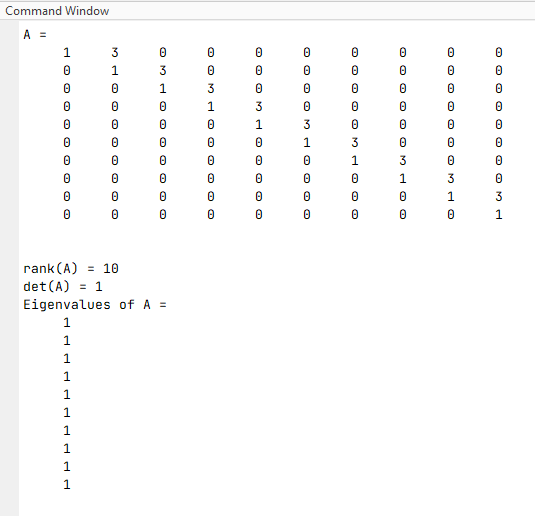
\includegraphics[width=9cm]{part3_1.png}
    \caption{Results from running matrix A of part III size 10x10 in MATLAB}
\end{figure}
\begin{figure}[ht]
    \centering
    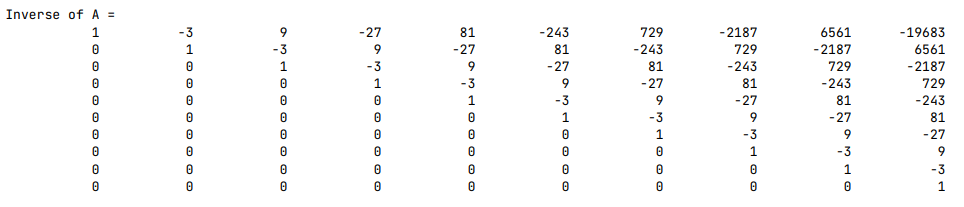
\includegraphics[width=\textwidth,height=\textheight,keepaspectratio]{Ainv_10x10.png}
    \caption{Inverse of matrix A of part III size 10x10}
\end{figure}
\begin{figure}[ht]
    \centering
    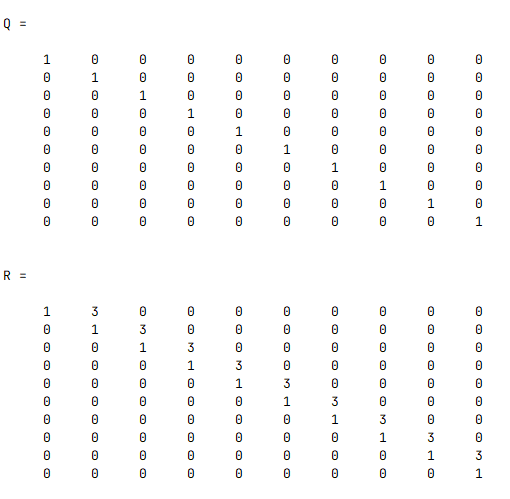
\includegraphics[width=12cm]{QR_part3.png}
    \caption{QR factorization of matrix A of part III size 10x10 in MATLAB}
\end{figure}
}

\end{document}